\section{Evaluation}
\label{sec:eval}

We conducted experiments on Planet-Lab platform to evaluate
SMON system. Planet-Lab is a global research network
consisting of 900+ nodes at 400+ sites around the
world.

%let SMON start self-deployment. We study the performance of
%the self-deployment process, and measure the overhead
%introduced in solving race conditions. To show SMON has
%good scalability, we deploy SMON on another set of 24
%nodes, and compare the performance with the previous
%deployment. We then close SMON by ... and study the
%performance ...
%
%Our experimental results show that SMON is efficient at
%deploying itself and achieves good scalability, the
%overhead caused by race condition is small and the active
%state transition is fast.

First, we evaluate the performance of self-deployment of
SMON.  We choose 159 nodes in Planet-Lab platform and start
a SMON peer. SMON then start deploying itself on all 159
nodes.

\begin{figure}
\centering
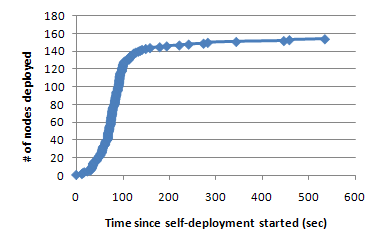
\includegraphics[scale=0.618]{self-deploy.png}
\caption{Progress of self-deployment process on 159
nodes.}
\label{fig:self-deploy}
\end{figure}

In our configuration, A SMON peer detects a random nodes and
sleep for 5 seconds. We finally collected data from 154
nodes out of 159 nodes. There are 5 nodes unreachable at
data-collecting stage and their data are omitted in the
result. This kind of failure is common for large scale
distributed systems.  Figure~\ref{fig:self-deploy} shows the
progress of self-deployment. We can see that 90\% (143) of
nodes are deployed successfully with a SMON peer within 149
seconds. The median deployment time is 93 seconds while the
largest one is 533 seconds. The long tail in
figure~\ref{fig:self-deploy} are caused by two reasons:
either the network to the machine is slow or the the machine
itself is overloaded and doesn't respond quickly.

We then evaluate the performance of enable/disable
self-management functionality of SMON system. We first
disable self-management of SMON system deployed on 159
Planet-Lab and then enable it again. The progress of state
transition from disabled to enabled is shown in
Figure~\ref{fig:state-transition}. For 90\%
percentile of peers, the states changes after 143
seconds and the median state transition time is 37 seconds.

\begin{figure}
\centering
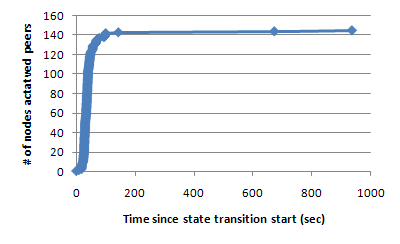
\includegraphics[scale=0.618]{state-trans.png}
\caption{Progress of state transition of self-management from disabled to
enabled.}
\label{fig:state-transition}
\end{figure}

%\begin{table}
%\centering
%\begin{tabular}{|l|c|}
%\hline
%median & 37 \\
%\hline
%90\% percentile & 143 \\
%\hline
%\end{tabular}
%\caption{Statistics for state transition experiment in seconds}
%\label{tbl:state-transition}
%\end{table}

To evaluate the scalability of self-deployment process, we deploy
a new instance of SMON system at a different scale (24 nodes) and
compare the performance of self-deployment process.
Table~\ref{tbl:scalability} summarizes the statistics results.
We can see from the table that the scalability is good.
While scale difference between two systems is about 6.6
(159/24) times, the
90-percentile deployment time is only 1.75 (149/85) times of
difference, while the median value is 1.41 (82/58) times of
difference.

\begin{table}
\centering
\begin{tabular}{|l|c|c|}
\hline
  & 24 nodes & 159 nodes\\
\hline
median & 58 sec & 82 sec \\
\hline
90\% percentile & 85 sec & 149 sec\\
\hline
Final & 103 sec & 533 sec\\
\hline
\end{tabular}
\caption{Comparison of self-deployment process at different
scales in seconds.}
\label{tbl:scalability}
\end{table}

During the self-deployment process, there are cases that
multiple SMON peers try to deploy an instance on the same
node and this can cause extra overhead. The overhead wastes
network bandwidth and the storage at the deployed node. We
evaluate the overhead by count the simultaneous deployment
happened at each node. The result is shown in
Figure~\ref{fig:overhead}. We can see that for 43.71\% of
nodes there is exactly one deployment on each of them.
Obviously, most of nodes have a deployment overhead within
10. These nodes account for 92.04\% of all nodes and the
average overhead of these nodes is 2.31. The average
overhead for all nodes is 4.30 which is an acceptable
number.

\begin{figure}
\centering
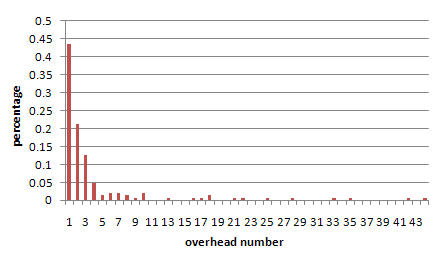
\includegraphics[scale=0.5]{overhead.png}
\caption{Overhead introduced by race condition during
self-deployment process}
\label{fig:overhead}
\end{figure}


% vim:foldmethod=marker:textwidth=60
